% LoVullo Specification Specification
%
% Yep.

\documentclass[draft]{lvspec}
\usepackage{multicol}
\usepackage[final]{graphicx}

\makeatletter
\makeatother

\begin{document}
\title[Lov2Spec]{LoVullo Specification Specifications}
\author{Mike Gerwitz}
\titlecontent{%
  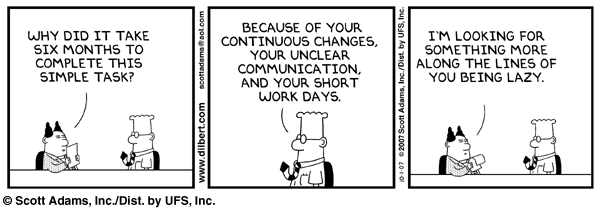
\includegraphics[scale=0.5]{images/dilbert-time.png}
  \vfill
}%
\abstract{%
  \setlength\columnsep{-5ex}%
  \begin{multicols}{2}
  \begin{quote}
    \sl\small\raggedright
    \def\ind{}%
    %
    In the beginning was the plan,\\
    \ind and then the specification;\\
    And the plan was without form,\\
    \ind and the specification was void.

    And darkness\\
    \ind was on the faces of the implementors thereof;\\
    And they spake unto their leader, saying:\\
    ``It is a crock of shit,\\
    \ind and smells as of a sewer.''

    And the leader took pity on them,\\
    \ind and spoke to the project leader:\\
    ``It is a crock of excrement,\\
    \ind and none may abide the odor thereof.''

    And the project leader\\
    \ind spake unto his section head, saying:\\
    ``It is a container of excrement,\\
    \ind and it is very strong, such that none may abide it.''

    The section head then hurried to his department manager,\\
    \ind and informed him thus:\\
    ``It is a vessel of fertilizer,\\
    \ind and none may abide its strength.''
    \goodbreak

    The department manager carried these words\\
    \ind to his general manager,\\
    and spoke unto him\\
    \ind saying:\\
    ``It containeth that which aideth the growth of plants,\\
    \ind and it is very strong.''

    And so it was that the general manager rejoiced\\
    \ind and delivered the good news unto the Vice President.\\
    ``It promoteth growth,\\
    \ind and it is very powerful.''

    The Vice President rushed to the President's side,\\
    \ind and joyously exclaimed:\\
    ``This powerful new software product\\
    \ind will promote the growth of the company!''

    And the President looked upon the product,\\
   \ind and saw that it was very good.

   \hfill---The Jargon File
  \end{quote}
  \end{multicols}
  \bigskip
}
\maketitle

\begindeptgroup{it}

\chapter{Oh, Hello}
\incomplete
\todo{There's no specification yet; in due time.}
\bigskip

\begin{center}
  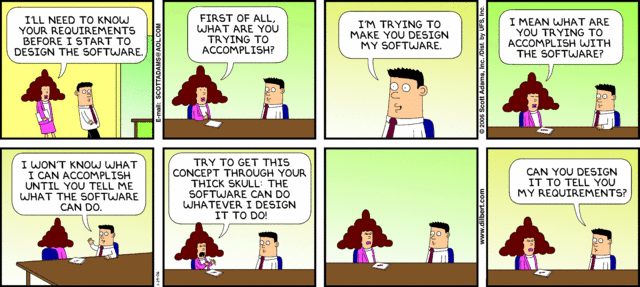
\includegraphics[scale=0.5]{images/spec-design.png}
\end{center}


\appendix
\chapter{Creating Specifications with \LaTeX}
This appendix is an example of an implementation of the specifications and is
useful as an API reference, but \shallnot be used in place of formal
specifications with regards to implementation.

Using the {\tt lvspec} document class with enable paragraph numbering; {\tt
draft} mode will enable signature lines, as shown to the right.

\begin{ex}
  \begin{verbatim}
% omit "[draft]" to disable signature lines
\documentclass[draft]{lvspec}

% as is the case with all LaTeX documents, begin and end with document
% environment
\begin{document}
  % ...content here...
\end{document}
  \end{verbatim}
\end{ex}

Example environments, as shown above, can be created with the {\tt ex}
environment. All examples end with `$\square$'.

\begin{ex}
  \begin{verbatim}
\begin{ex}
  % ...example here...
\end{ex}
  \end{verbatim}

  The extra vertical space is simply because of the \cmd{verbatim} environment
  used for the above examples; \cmd{ex} itself does not add it, as shown here.
\end{ex}


\section{General Formatting}
There are a number of formatting decisions that \cmd{lvspec} makes for you; you
should \emph{not} override them manually, since the \cmd{lvspec}~class is
intended to provide a company-wide abstraction that can be easily modified to
apply to all specifications.

The \cmd{lvspec}~class is based on the \cmd{scrreprt}~class, which is in turn
very similar to the standard \LaTeX\ \cmd{report}~class. In particular, all
section levels starting with \verb|\chapter| are supported and margins are of
equal length on both sides, which is suitable for collating portions of the
document without having to worry about binding and what side a particular page
is printed on. Margins are large to provide plenty of space for annotations and
reader markup. The default page size is US~letter.

\cmd{lvspec} suppresses paragraph indentation and instead adds space between
paragraphs, which is more natural with paragraph numbering (see~\sref{parnum}).

The amount of text on a page is determined by a ratio that carefully balances
characters per line and number of lines on a page according to established
typesetting conventions and also takes into account Hermann~Zapf's ideas for
page ``grayness'' (where a page appears darker with more text). Since
\cmd{lvspec} adds additional whitespace between lines, it accommodates by
decreasing the height of the top and~bottom page margins. Furthermore, glue
between section headings has been condensed slightly and is not as stretchable.

The header of each page contains the document title (short title if provided) in
the upper-right hand corner, with the current section (as of the beginning of
the page) on the upper-left. The typeface is in {\sc Small Caps} to distinguish
it from the page body which is in fairly close proximity. The font size has also
been {\small slightly decreased} to move focus away from it.

\p{ex:footer}
The footer of each page contains, from left to right, the section number of the
last section to appear on the page; the current page number; and a unique
version identifier that is either taken from \path{verstr.tex} or---if
unavailable---the current date.\footnote{See \path{lvspec.git/Makefile} for an
example of how to use \path{verstr.tex}.}

Section numbers are enabled for sub-subsections.


\subsection{Title Page and Abstract}
The title is typeset in {\sc Small Caps} to provide stronger emphasis than a
normal typeface (because {\bf bold is too bold}).

If the \cmd{draft} option is provided via \verb|\documentclass|, then the text
``{\sc(Working Draft)}'' will be typeset below the title.

The \verb|\title| command is modified to support an optional ``short title'' to
be used primarily in the header to provide additional space for section names.

The text ``{\sc LoVullo Associates}'' is added below any provided author(s).

The date of document generation is typeset flush with the bottom of the page
body.

Two bold, vertical bars span the entire length of the page body in the left and
right margins.

Additional content may be added to the title page below the author and above the
date by using the \verb|\titlecontent| command.

An abstract may be typeset on the following page using the~\verb|\abstract|
command. If the~\cmd{draft} option is provided, an additional paragraph will be
added---regardless of whether an abstract was given---stating that the document
is a draft.

Flush with the bottom of the abstract page body is a copyright notice, date of
page generation (the same date that appears on the title page) and the version
identifier that appears on the footer of every page (as mentioned
in~\pref{ex:footer}).

\begin{ex}
  \begin{verbatim}
\begin{document}
\title[Lov2Spec]{LoVullo Specification Specifications}
\author{Mike Gerwitz}
\titlecontent{%
  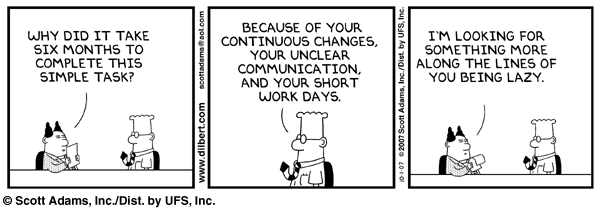
\includegraphics[scale=0.5]{images/dilbert-time.png}
  \vfill
}%
\abstract{...}
\maketitle
% ...
  \end{verbatim}
\end{ex}

Immediately after the title and~abstract pages are typeset, paragraph numbering
(see~\sref{parnum}) and~signature lines (see~\sref{siglines}) are enabled.

\section{Paragraph Numbering}\label{s:parnum}
Paragraph numbering can be temporarily disabled using \verb|\pnumoff| and
re-enabled using \verb|pnumon|\ldots

\pnumoff
\ldots as shown here.

\pnumon
Numbers will continue where they previously left off before being suppressed.

\begin{ex}
  \begin{verbatim}
Paragraph numbering can be temporarily disabled using \verb|\pnumoff| and
re-enabled using \verb|pnumon|\ldots

\pnumoff
\ldots as shown here.

\pnumon
Numbers will continue where they previously left off before being suppressed.
  \end{verbatim}
\end{ex}

Disabling paragraph numbering also disables the signature line, since there is
no longer any disambiguating identifier.

\begin{itemize}
  \item Paragraph numbering, by default, does not take effect inside any
  environments.\footnote{Except for \cmd{document}.}
\end{itemize}

\begin{ex}
  \begin{verbatim}
\begin{itemize}
  \item Paragraph numbering, by default, does not take effect inside any
  environments.\footnote{Except for \cmd{document}.}
\end{itemize}
  \end{verbatim}
\end{ex}


\section{Signature Lines}\label{s:siglines}
The department for the entire section can be set using the
\verb|\sectiondept| command; the command takes effect until the next section
or chapter.

\begin{ex}
  \begin{verbatim}
\section{Signature Lines}
\sectiondept{it}
The department for the entire section can be set using the
\verb|\sectiondept| command; the command takes effect until the next section
or chapter.
  \end{verbatim}
\end{ex}

\dept{pm}
The department can be set per-paragraph using the \verb|\dept| command, as
demonstrated in this paragraph; the command will override any
\verb|\sectiondept| command temporarily and will undo itself after the paragraph
ends.

\begin{ex}
  \begin{verbatim}
\dept{pm}
The department can be set per-paragraph using the \verb|\dept| command, as
demonstrated in this paragraph; the command will override any
\verb|\sectiondept| command temporarily and will undo itself after the paragraph
ends.
  \end{verbatim}
\end{ex}

\dept{it}
An arbitrary group of paragraphs may have their section set using
\verb|\begindeptgroup| and \verb|\enddeptgroup|; they are \emph{not} reset by
sections. They may be nested.

\begin{ex}
  \begin{verbatim}
\begindeptgroup{it}
  % group: it
  \begindeptgroup{pm}
    % group: pm
  \enddeptgroup
  % group: it
\enddeptgroup
  \end{verbatim}
\end{ex}

Clicking on the department in the signature line will take you to the
^[authorization parties] section of the definitions (in this document,
\sref{authorize}).

All unauthorized paragraphs are added to the index under the heading of
``{\bf Needs Authorization}'' to ensure that nothing is missed, boldfaced to
make the problem apparent.

\subsection{Incomplete}
\incomplete
If a paragraph is incomplete and not yet ready for authorization, use
\verb|\incomplete|.

\begin{ex}
  \begin{verbatim}
\incomplete
If a paragraph is incomplete and not yet ready for authorization, use
\verb|\incomplete|.
  \end{verbatim}
\end{ex}

\incompletei
If a paragraph is incomplete because more information is needed, then use the
command \verb|\incompletei|, which also includes the name of the department.

\begin{ex}
  \begin{verbatim}
\incompletei
If a paragraph is incomplete because more information is needed, then use the
command \verb|\incompletei|, which also includes the name of the department.
  \end{verbatim}
\end{ex}

All incomplete paragraphs are added to the index under the heading of
``{\bf Incomplete}'' to ensure that nothing is missed, boldfaced to make the
problem apparent.



\section{Definitions}
The formal language of the specification is important to resolve any
ambiguities; part of such a resolution involves the formal and unambiguous
definition of terms.

\begin{center}
  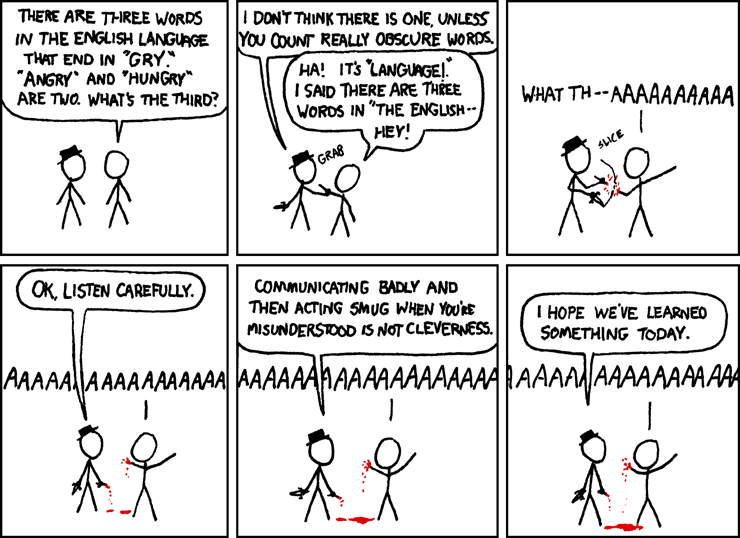
\includegraphics[width=0.8\textwidth]{images/words_that_end_in_gry.png}
\end{center}

\pnumon
By default, \cmd{lvspec} will \emph{always} include specification definitions
(see~\sref{specdfn}).

When the~\cmd{draft} option is provided, a~section describing authorization
parties will also be added, which is linked to by the department in each
signature line.

Additionally, the following options may be provided via~\verb|\documentclass|:

\begin{description}
  \item[\cmd{devterms}]
  Comprehensive developer terminology that covers specifications that deal with
  software and/or~hardware details.

  \item[\cmd{insuranceterms}]
  General insurance terminology to be used in any specification that describes
  an insurance-related implementation. Additional content can be added
  immediately after the terms (e.g. to add a sub-section) by using the command
  \verb|\insuranceterminology|, which is only available if
  the~\cmd{insuranceterms} option is used.
\end{description}

% TODO: this \pnumon won't be needed once sPxTeX is used, as it does not have
% this problem
\pnumon
Additional sections can be added before\footnote{Ensures that section numbers do
not change by disabling \cmd{draft} mode.} the authorization party sub-section
(or, if the~\cmd{draft} option is not provided, then at the end of the
definitions section) by using the \verb|\terminology| command.

The definitions section is not a substitute for an English dictionary for
undefined terms.

\begin{center}
  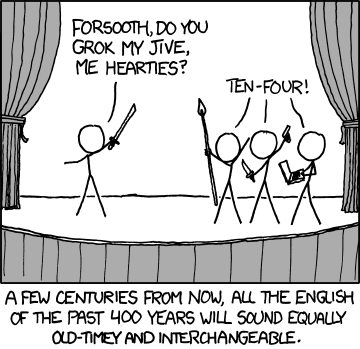
\includegraphics[width=0.7\textwidth]{images/period_speech.png}
\end{center}
\pnumon


\section{Table of Contents, Index and Bibliography}
A table of contents will be output after the title and abstract pages and will
include up to sub-subsections in depth. Furthermore, a mini table of contents
will be output after every chapter heading.

If a chapter contains figures or tables, then a list of figures and/or~a list of
tables will be output, respectively, after the mini table of contents.

A bibliography will be output if the~\verb|\cite| command is used at least once.
By default, the file~\path{common.bib} will be used.

\subsection{Index}
A well-structured and complete index is considered to be a sign of an organized
and well-authored work. You should pay attention to your index, as it helps
people find things, even if searching is available (e.g. in PDF~form).

An index will be output at the end of the document. Certain commands
(e.g.~\verb|\dfn|) add to the index automatically, but other entries must be
manually added throughout the text using \verb|\index|.

\begin{ex}
  \begin{verbatim}
This paragraph is about \index{animals!cats}cats.

\section{Cats}
\index{animals!cats|(}
% ...
This whole section is about cats!
% ...
\index{animals!cats|)}

This section is \emph{not} about cats.
  \end{verbatim}
\end{ex}

The command \verb|\dfn| accepts a more primitive index syntax (supporting~`!'),
formats the command as a~\dfn{definition}, and displays the text after the
rightmost~`!', or the entire text if no such character exists.

\begin{ex}
  \begin{verbatim}
% the following two paragraphs are equivalent
This paragraph is about \index{animals!cats}cats.

% the only difference is that ``cats'' is styled in this paragraph, but not
% above
This paragraph is about \dfn{animals!cats}.
  \end{verbatim}
\end{ex}

A limited short-hand notation, inspired by Knuth's \TeX{}book, is also
available: The `\^{}' character has been re-mapped as a command and will take
the word that follows it and place it into the index (in addition to typesetting
it). If the word contains spaces, then it may be enclosed in brackets. The
`\^{}' character retains it original meaning within math mode (e.g. $4\pi r^2$).

\begin{ex}
  \begin{verbatim}
In this paragraph, ``^word'' is placed into the index, as well as ``^[multiple
words]''.

The `\^{}' character retains it original meaning within math mode
(e.g. $4\pi r^2$).
  \end{verbatim}
\end{ex}


\section{Miscellaneous}
% text has been carefully added to this line; margin, font, etc changes will
% ruin it!
Proper hyphenation is added for ``ConceptOne'', as is shown here on this line:
ConceptOne test.

\enddeptgroup


\pnumoff
\chapter{\LaTeX\ Tips}
This appendix is by no means comprehensive.

\section{Generating PDF}
A PDF can be generated from the~\TeX\ source files by issuing the command
\cmd{pdflatex}; indexes are generated using the command \cmd{makeidx}; and
bibliographies are generated using \cmd{bibtex}. First, \cmd{pdftex} must be run
to determine the page numbers and gather all the references. Then, after each of
the latter two commands are run, \cmd{pdftex} must be re-run in order to update
the document. Since the act of updating the document may alter the references,
it is recommended to run \cmd{pdftex} multiple times at the end:\footnote{See
\path{lvspec.git/Makefile} for an example.}

\begin{ex}
  \begin{verbatim}
$ pdftex src.tex \
> && bibtex src.tex \
> && makeindex src \
> && pdftex src.tex \
> && pdftex src.tex
  \end{verbatim}
\end{ex}

\noindent You may decide to omit \cmd{bibtex} if you are not using a
bibliography (but you probably should cite your information and rationale).

\end{document}
